\documentclass[11pt, a4paper]{report}

\usepackage{fullpage}
% A more tightly packed list than the standard
% \enumerate{itemize} append * after enumeration type
\usepackage{mdwlist}
% Multi-page tables + accompanying header and footer comments
\usepackage{longtable}

% Vertical table headers, not sure what does what. graphicx is
% multi-purpose and does a lot of other stuff like including images
\usepackage{array,graphicx}
\usepackage{booktabs}

% Lossless .png format expected for figures
\DeclareGraphicsExtensions{.png}

% \verbatiminput command (\begin{verbatim} is standard lib)
\usepackage{verbatim}

\newcommand*\rot{\rotatebox{90}}


\title{Modeling an Online Music Business}
\author{Zane Kansil\\ Loyola Marymount University\\ Database Systems}

% Allow commands
\providecommand\phantomsection{}

% Custom ToC labeling
\renewcommand\thechapter{\Roman{chapter}}
\renewcommand\thesection{\thechapter.\arabic{section}}

% Custom ToC spacing between chapter number and
% chapter name
\usepackage{tocloft}
\setlength{\cftchapnumwidth}{3em}
\setlength{\cftsecnumwidth}{3.5em}
\setlength{\cftsubsecnumwidth}{4em}

\begin{document}

%---    Title page    ---%
\clearpage
\phantomsection
\addcontentsline{toc}{chapter}{%
    \protect\numberline{I}Title Page}
\maketitle

%---    ToC    ---%
\clearpage
\phantomsection
\addcontentsline{toc}{chapter}{%
    \protect\numberline{II}Contents}
\tableofcontents
% The title page and ToC are difficult to handle,
% we set the page and chapter counter after the
% ToC is generated so that the rest of the document
% can continue on from there.
\setcounter{page}{2}
\setcounter{chapter}{2}

%---    Description of the Enterprise    ---%
\chapter{Description of the Enterprise}
A friend of mine intends to put out an all­-purpose site for his musical career. The site will be a hub for his online business and allow him to track sales and interactions with his fans.\\

The site will serve as a place to feature embedded music and video players for John's music. It will be necessary to monitor this hosted media in terms of listens and views. Some other metrics John is interested in are on­-site plays (not a redirect), and redirects to his Soundcloud and YouTube accounts from their embedded players on his site. Videos and Songs are tracked separately due to their differing properties.\\

There is a sales aspect to the site, merchandise will also be sold under the same domain. Some
merchandise will be physical, such as hats, headbands, wristbands and stickers. Other merchandise
will be digital, such as a donation to download a mixtape (a non-album collection of John's music). Physical merchandise needs to be shipped, so appropriate data such as \texttt{shipping\_status} and \texttt{destination} will need to be tracked. With physical merchandise, quantity and availability must be tracked. Digital merchandise is easier to manage as it is transmitted and there is less customer data to collect. Digital merchandise will also be
infinitely available if listed, so there is no quantity­ related data to track.\\

JohnDB records data for Physical and Digital consumers separately.\\

As the main operator of his business, John wants to track of his sales and revenue. The most simple way to track this would be through a table of sales records. These records would detail everything necessary about the sale. A sale would correspond to a single type of product. If multiple products were purchased in the same transaction, then multiple sale entries would be logged.\\

\clearpage
\section{Ten sample Questions John would ask}
\begin{enumerate}
    \item How many video plays today?
    \item How many redirects to Soundcloud from embedded music players?
    \item What is the redirect rate for videos?
    \item Is ``Black Silk Hooded Sweatshirt'' sold out?
    \item How many ``Red Summer Beanie'' items were sold in October 2014?
    \item What physical goods are currently frozen? (sales prevented)
    \item How many orders do I have to fill to the US?
    \item What precentage of my digital consumers are from outside the US?
    \item What is the average monthly revenue over the past six months?
    \item What products have garnered zero sales in the past 14 days? 
\end{enumerate}

%---    Definition of Environment    ---%
\chapter{Definition of Environment}

\section{Input and Report forms}

% Number forms
\begin{enumerate}
\item Video Metadata View
    % itemize* is a more compacted list
    % imported by mdwlist
    \begin{itemize*}
      \item Video Name
      \item Video (hosted at) URL
      \item Number of plays
      \item Total plays
      \item Plays Today
      \item Plays Yesterday
      \item Total redirects to YouTube
    \end{itemize*}

\item Song Metadata View
    \begin{itemize*}
      \item Song Name
      \item Song Artist
      \item Song (hosted at) URL
      \item Total plays
      \item Plays Today
      \item Plays Yesterday
      \item Total redirects to SoundCloud
    \end{itemize*}

\item Add New Physical good
    \begin{itemize*}
      \item Name
      \item Description Paragraph
      \item Upload/Choose an Image
      \item Color (optional)
      \item Size (optional)
      \item Price (in USD)
      \item Current stock on hand
    \end{itemize*}

\item Add New Digital good
    \begin{itemize*}
      \item Name
      \item Description Paragraph
      \item Upload/Choose an Image
      \item Price (in USD)
    \end{itemize*}

\item Physical Good Admin
    \begin{itemize*}
      \item Name (editable)
      \item SKU (generated from original name, can re-generate)
      \item Description Paragraph (truncated, editable)
      \item Image (editable)
      \item Color (editable)
      \item Price (editable)
      \item Quantity Available (editable, warning message)
      \item Total sales
    \end{itemize*}

\item Digital Good Admin
    \begin{itemize*}
      \item Name (editable)
      \item SKU (generated from original name, can re-generate)
      \item Description Paragraph (truncated, editable)
      \item Image (editable)
      \item Price (editable)
      \item Freeze sales (boolean, editable, default false)
    \end{itemize*}

\item Physical Consumer details entry
    \begin{itemize*}
      \item First Name
      \item Last Name
      \item Email
      \item Phone (optional)
      \item Address Line 1
      \item Address Line 2 (optional)
      \item Zip Code
      \item Country (un-settable, value is ‘US’)
      \item State (dropdown)
    \end{itemize*}

\item Digital Consumer details entry
    \begin{itemize*}
      \item First Name
      \item Last Name (optional)
      \item Email
      \item Phone (optional)
      \item Country
    \end{itemize*}

\item Sales table
    \begin{itemize*}
      \item Item id
      \item Item SKU
      \item Sale type (\texttt{digital} or \texttt{physical})
      \item Status (\texttt{received}, \texttt{shipped} or \texttt{fulfilled})
      \item Quantity
      \item Unit Price
      \item Total Order Cost
      \item Date received
    \end{itemize*}
 
\end{enumerate}

\clearpage
\section{Assumptions}
\begin{enumerate}
\item Forms are used to add items to the site
\item Tables as opposed to graphs are the prefered way to view data
\item The Sales table functions as an Orders table as well, showing the status of each order in addition to transaction information
\item Only customers in the ‘US’ are allowed to order physical goods
\end{enumerate}

\clearpage
\section{User-oriented data dictionary}

\begin{longtable}{|l|l|l|l|l|l|l|l|l|l|}

\hline
\multicolumn{1}{|c|}{Datum} &
\multicolumn{9}{c|}{Form or Screen} \\[1ex]

\hline
& \rot{Video Metadata View} &
\rot{Song Metadata View} &
\rot{Add New Physical good} &
\rot{Add New Digital good} &
\rot{Physical Good Admin} &
\rot{Digital Good Admin} &
\rot{Physical Consumer details entry} &
\rot{Digital Consumer details entry} &
\rot{Sales table} \\
\hline

dc\_country             &                &   &   &   &   & x &   & x &   \\ \hline
dc\_first\_name         &                &   &   &   &   & x &   & x &   \\ \hline
dc\_id                  &                &   &   &   &   & x &   &   &   \\ \hline
dc\_last\_name          &                &   &   &   &   & x &   & x &   \\ \hline
dc\_phone               &                &   &   &   &   & x &   & x &   \\ \hline
dg\_description         &                &   &   & x &   &   &   &   &   \\ \hline
dg\_image               &                &   &   & x &   &   &   &   &   \\ \hline
dg\_is\_available       &                &   &   & x &   &   &   &   &   \\ \hline
dg\_name                &                &   &   & x &   &   &   &   &   \\ \hline
dg\_price               &                &   &   & x &   &   &   &   &   \\ \hline
dg\_sales               &                &   &   & x &   &   &   &   &   \\ \hline
dg\_sku                 &                &   &   & x &   &   &   &   & x \\ \hline
mv\_plays               & x              &   &   &   &   &   &   &   &   \\ \hline
mv\_plays\_today        & x              &   &   &   &   &   &   &   &   \\ \hline
mv\_plays\_yesterday    & x              &   &   &   &   &   &   &   &   \\ \hline
mv\_redirects           & x              &   &   &   &   &   &   &   &   \\ \hline
mv\_title               & x              &   &   &   &   &   &   &   &   \\ \hline
mv\_upload\_date        & x              &   &   &   &   &   &   &   &   \\ \hline
mv\_url                 & x              &   &   &   &   &   &   &   &   \\ \hline
pc\_address\_line\_1    &                &   &   &   & x &   & x &   &   \\ \hline
pc\_address\_line\_2    &                &   &   &   & x &   & x &   &   \\ \hline
pc\_country             &                &   &   &   & x &   & x &   &   \\ \hline
pc\_email               &                &   &   &   & x &   & x &   &   \\ \hline
pc\_first\_name         &                &   &   &   & x &   & x &   &   \\ \hline
pc\_id                  &                &   &   &   & x &   &   &   &   \\ \hline
pc\_last\_name          &                &   &   &   & x &   & x &   &   \\ \hline
pc\_phone               &                &   &   &   & x &   & x &   &   \\ \hline
pc\_state               &                &   &   &   & x &   & x &   &   \\ \hline
pc\_zip\_code           &                &   &   &   & x &   & x &   &   \\ \hline
pg\_color               &                &   & x &   &   &   &   &   &   \\ \hline
pg\_description         &                &   & x &   &   &   &   &   &   \\ \hline
pg\_image               &                &   & x &   &   &   &   &   &   \\ \hline
pg\_name                &                &   & x &   &   &   &   &   &   \\ \hline
pg\_price               &                &   & x &   &   &   &   &   &   \\ \hline
pg\_quantity\_available &                &   & x &   &   &   &   &   &   \\ \hline
pg\_sales               &                &   &   &   &   &   &   &   &   \\ \hline
pg\_size                &                &   & x &   &   &   &   &   &   \\ \hline
pg\_sku                 &                &   & x &   &   &   &   &   & x \\ \hline
sa\_digital\_sale       &                &   &   &   &   &   &   &   & x \\ \hline
sa\_filfill\_date       &                &   &   &   &   &   &   &   & x \\ \hline
sa\_id                  &                &   &   &   &   &   &   &   & x \\ \hline
sa\_physical\_sale      &                &   &   &   &   &   &   &   & x \\ \hline
sa\_price               &                &   &   &   &   &   &   &   & x \\ \hline
sa\_quantity            &                &   &   &   &   &   &   &   & x \\ \hline
sa\_sku                 &                &   &   &   &   &   &   &   & x \\ \hline
sa\_status              &                &   &   &   &   &   &   &   & x \\ \hline
sa\_timestamp           &                &   &   &   &   &   &   &   & x \\ \hline
sa\_total\_cost         &                &   &   &   &   &   &   &   & x \\ \hline
so\_artist              &                & x &   &   &   &   &   &   &   \\ \hline
so\_plays               &                & x &   &   &   &   &   &   &   \\ \hline
so\_plays\_today        &                & x &   &   &   &   &   &   &   \\ \hline
so\_plays\_yesterday    &                & x &   &   &   &   &   &   &   \\ \hline
so\_redirects           &                & x &   &   &   &   &   &   &   \\ \hline
so\_title               &                & x &   &   &   &   &   &   &   \\ \hline
so\_upload\_date        &                & x &   &   &   &   &   &   &   \\ \hline
so\_url                 &                & x &   &   &   &   &   &   &   \\ \hline

\end{longtable}

\clearpage
\section{Cross-reference table}
Incomplete?

%---    Enterprise Database Design    ---%
\chapter{Enterprise Database Design}

\section{Logical model of the Enterprise}

\subsection{List of Entities and Attributes}

\begin{enumerate}

\item Media
    \begin{itemize*}
      \item m\_id
    \end{itemize*}

\item Music Video
    \begin{itemize*}
      \item mv\_title
      \item mv\_url                              (url video is hosted at)
      \item mv\_upload\_date
    \end{itemize*}

\item Song
    \begin{itemize*}
      \item so\_title
      \item so\_artist
      \item so\_url                              (url song is hosted at)
      \item so\_upload\_date
    \end{itemize*}

\item Interaction
    \begin{itemize*}
      \item i\_date
    \end{itemize*}

\item Play

\item Redirect
    \begin{itemize*}
      \item to              (``YouTube'' or ``SoundCloud'')
    \end{itemize*}

\item Consumer
    \begin{itemize*}
      \item c\_id
      \item c\_firstname
      \item c\_lastname
      \item c\_email
    \end{itemize*}

\item Physical Consumer
    \begin{itemize*}
      \item pc\_address\_line\_1
      \item pc\_address\_line\_2
      \item pc\_country
      \item pc\_state
      \item pc\_phone
    \end{itemize*}

\item Digital Consumer
    \begin{itemize*}
      \item dc\_phone                        (for confirmation, optional)
      \item dc\_country                      (optional)
    \end{itemize*}

\item Purchase
    \begin{itemize*}
      \item sale\_id
      \item sale\_date              (datetime)
      \item sale\_status            is Received, Shipped or Fulfilled
    \end{itemize*}

\item Line Item
    \begin{itemize*}
      \item quantity
    \end{itemize*}

\item Good
    \begin{itemize*}
      \item g\_sku
      \item g\_name
      \item g\_description
      \item g\_price
    \end{itemize*}

\item Digital Good
    \begin{itemize*}
      \item dg\_is\_frozen            (boolean, used to prevent ordering)
    \end{itemize*}

\item Physical Good
    \begin{itemize*}
      \item pg\_color
      \item pg\_size
      \item pg\_quantity\_available
    \end{itemize*}

\end{enumerate}

* - A datetime is an instant in time. Has date information and time-of-day information. Example: 2014-09-06T15:35:58+00:00 (September 6, 2014, 3:35:58pm)

\clearpage
\subsection{List of Relationships and Attributes}

\noindent\textbf{Media Relationships}
\begin{enumerate}
\item MUSIC\_VIDEO has many INTERACTION
\item INTERACTION has 1 MUSIC\_VIDEO
\item SONG has many INTERACTION
\item INTERACTION has 1 SONG
\item INTERACTION is a PLAY
\item INTERACTION is a REDIRECT
\end{enumerate}

\noindent\textbf{Sales Relationships}
\begin{enumerate}
\item CONSUMER is a PHYSICAL\_CONSUMER
\item CONSUMER is a DIGITAL\_CONSUMER
\item CONSUMERS make many PURCHASE
\item PURCHASE has 1 CUSTOMER
\item PURCHASE has many LINE\_ITEM
\item PURCHASE has 1 STATUS
\item STATUS is applicable to 1 PURCHASE
\item LINE\_ITEM belongs to 1 PURCHASE
\item LINE\_ITEM has 1 GOOD
\item GOOD can appear in many LINE\_ITEM
\item GOOD is a DIGITAL\_GOOD
\item GOOD is a PHYSICAL\_GOOD
\end{enumerate}

\clearpage
\subsection{Entity-Relationship diagram of the Enterprise}
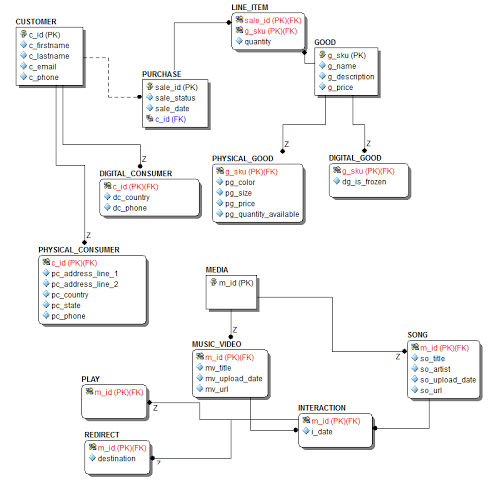
\includegraphics[]{ERB.png}
-ZK: will upgrade resolution next time...

\clearpage
\section{Conceptual model of the enterprise}

\begin{verbatim}
MEDIA(m_id)

MUSIC_VIDEO(m_id, mv_title, mv_url, mv_upload_date)
    PK/FK: m_id
    CK: m_id, mv_title, mv_url

SONG(m_id, so_title, so_artist, so_url, so_upload_date)
    PK/FK: m_id
    CK: m_id, so_title, so_url

PLAY(m_id, i_datetime)
    PK/FK: m_id
    CK: m_id

REDIRECT(m_id, m_to)
    PK/FK: m_id
    CK: m_id

CONSUMER(c_id, c_firstname, c_lastname, c_email)
    PK: c_id
    CK: c_id, c_email

PHYSICAL_CONSUMER(
  c_id
, pc_address_line_1
, pc_address_line_2
, pc_country
, pc_state
, pc_phone
)
    PK/FK: c_id
    CK: c_id, pc_phone

DIGITAL_CONSUMER(
  c_id
, pc_phone
, pc_country
)
    PK/FK: c_id
    CK: c_id, pc_phone

PURCHASE(p_id, c_id, p_date)
    PK/FK: p_id
    CK: p_id, c_id



LINE_ITEM(p_id, g_id, quantity)
    PK: p_id
    CK: p_id
    FK: p_id, g_id

GOOD(g_name, g_description, g_sku, g_price)
    PK: g_sku
    CK: g_name, g_sku

DIGITAL_GOOD(g_sku, dg_is_frozen)
    PK: g_sku
    CK: g_sku

PHYSICAL_GOOD(g_sku, pg_color, pg_size, pg_quantity_available)
    PK/FK: g_sku
    CK: g_sku
\end{verbatim}

\clearpage
\section{Table dictionary}

\clearpage
\section{Attribute dictionary}

%---    Database and Query Definition    ---%
\chapter{Database and Query Definition}

\section{Database Definition}
    \verbatiminput{online-music-business.sql}

\clearpage
\section{Database Queries}
    \verbatiminput{db-queries-10-questions.sql}

\clearpage
\section{Design Tradeoffs and Limitations}
Not too many limitation currently. I recently added a parent \texttt{MEDIA} entity for videos and songs.

%---    Database Integrity and Security    ---%
\chapter{Database Integrity and Security}
\section{Functional Dependencies}
    A list of the functional dependencies that hold on your database.
\section{Adjustments for Normalization}
    An explanation of the changes needed to normalize your database.
\section{Integrity and Security}
    A list (in English) of the integrity and security constraints which are to hold on your database.

%---    Implementation Notes    ---%
\chapter{Implementation Notes}
\section{Indices}
    A list of the indices used by your database, with a justification for each.
\section{Data}
    The data used to populate your database.
\section{Query Trace}
    A trace of the execution of each of your queries.
\section{Implementation Assessment}
    An assessment of how smoothly your implementation went

%---    Lessons Learned    ---%
\chapter{Lessons Learned}

\end{document}
